\section{Etwas zu Essen. Bedingungen, Variablen, Ausblenden, and Sound.}

\subsection{Erzeuge das Essen!}
\begin{itemize}

\item[1.] Wähle ein neues Sprite aus einer Datei. Wir haben einen Ball gewählt, du kannst jedoch auch etwas anderes nehmen oder sogar selber zeichnen.
\end{itemize}
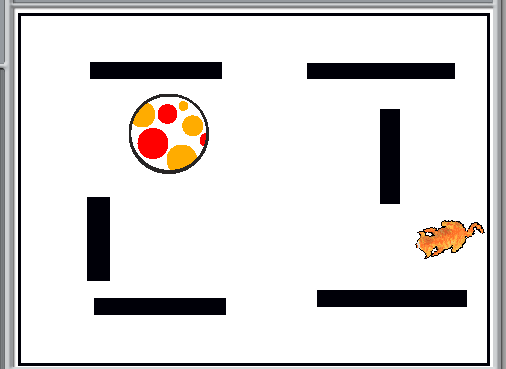
\includegraphics[width=0.6\textwidth]{images/aufgabe3_uebersicht.png}
\begin{itemize}
\item[2.] Benutze das Verkleinerungs-Tool, um die Größe deines Sprites in Relation zum Rest zu bringen.
\end{itemize}
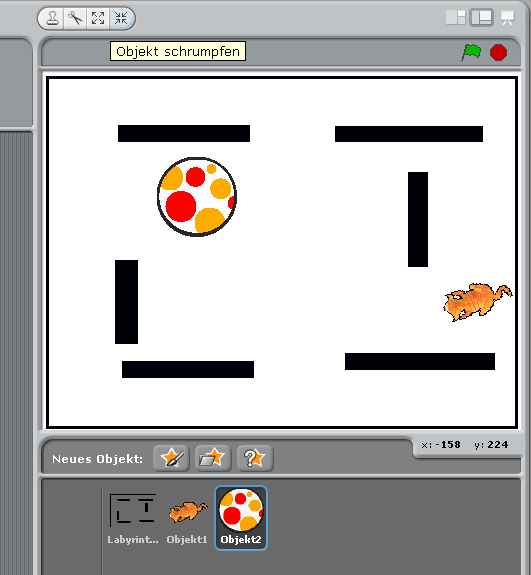
\includegraphics[width=0.6\textwidth]{images/aufgabe3_schrumpfen.png} \newline
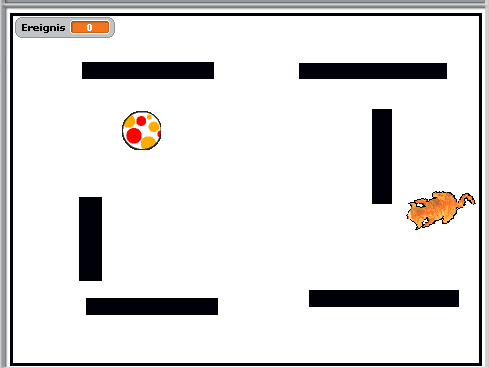
\includegraphics[width=0.6\textwidth]{images/aufgabe3_schrumpfen2.png}
\begin{itemize}
\item[3.] Benenne dein Sprite um. Meins heißt \textit{Ball}.
\end{itemize}]

\subsection{Erzeuge das Skript für das Ergebnis und das Ausblenden}

\begin{itemize}
\item[4.] Klicke auf \textit{Variablen} und auf \textit{Neue Variable}, nenne Sie \textit{Ergebnis} und klicke auf \textit{OK}.
\end{itemize}
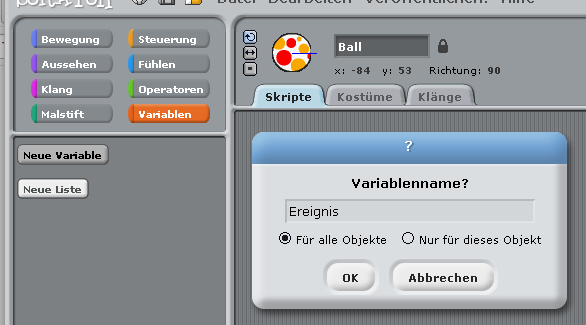
\includegraphics[width=0.6\textwidth]{images/aufgabe3_variable.png}
\begin{itemize}
\item[5.] Ziehe aus dem Steuerungs-Panel, die \textit{Wenn grüner Pfeil angeklickt} und die \textit{wiederhole fortlaufen}-Kachel in das Skript-Panel und verbinde beide.
\end{itemize}
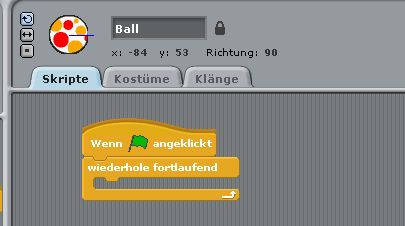
\includegraphics[width=0.6\textwidth]{images/aufgabe3_ball1.png}
\begin{itemize}
\item[6.] Füge folgendes noch hinzu:
\subitem Setze das Ergebnis auf 0 und füge es zwischen der \textit{Wenn grüner Pfeil geklickt} und \textit{wiederhole fortlaufend} ein.
\subitem Füge aus dem Fühlen-Panel die \textit{wird berührt}-Kachel in die Wabe der \textit{wiederhole fortlaufend}-Kachel ein.
\subitem Füge in die Freie Fläche der \textit{wiederhole fortlaufend}-Kachel aus dem Variablen-Panel die \textit{ändere Ergebnis um 1}-Kachel ein.
\end{itemize}
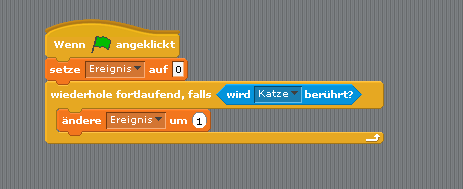
\includegraphics[width=0.6\textwidth]{images/aufgabe3_ball2.png}
\begin{itemize}
\item[7.] Füge nun aus dem Aussehen-Panel eine \textit{zeige dich} und \textit{verstecke dich}-Kachel hinzu.
\subitem Die \textit{zeige dich}-Kachel direkt unter das \textit{Wenn grüner Pfeil geklickt} und \textit{Setze Ergebnis auf 0}.
\subitem Die \textit{verstecke dich}-Kachel unterhalb \textit{ändere Ergebnis um 1}
\end{itemize}
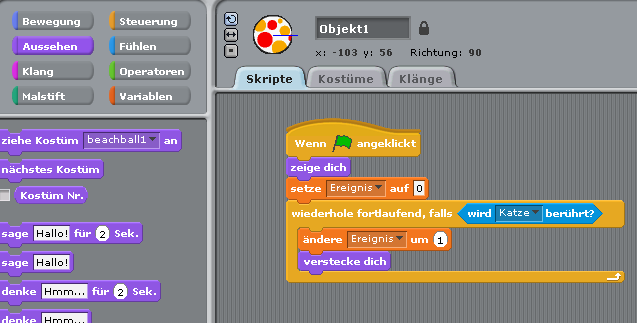
\includegraphics[width=0.6\textwidth]{images/aufgabe3_ball2b.png}
\begin{itemize}
\item[8.] Überprüfe deine Einstellung mit dem Bild und klicke auf den grünen Pfeil.
\item[9.] Der Ball sollte ausgeblendet werden und das Ergebnis um 1 erhöht sein.
\end{itemize}

\subsection{Füge einen Klang hinzu, wenn der Ball deinen Sprite berührt}
\begin{itemize}
\item[10.] Klicke auf deine Figur und wähle den Klang-Panel.
\end{itemize}
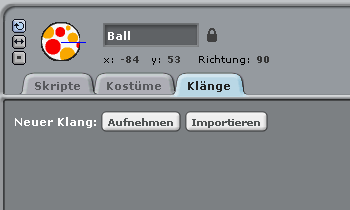
\includegraphics[width=0.6\textwidth]{images/aufgabe3_ton1.png}
\begin{itemize}
\item[11.] Klicke auf Importieren und wähle einen Klang aus der Ordnerliste.
\end{itemize}
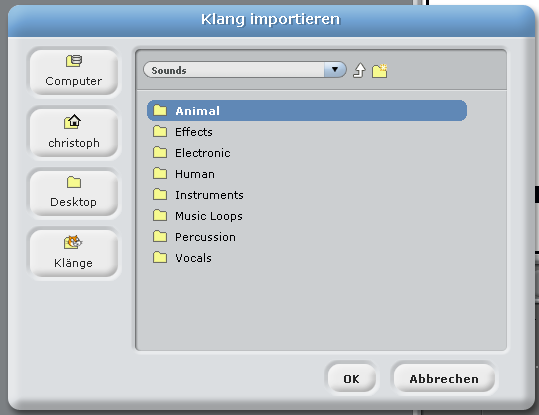
\includegraphics[width=0.6\textwidth]{images/aufgabe3_ton2.png} 
\begin{itemize}
\item[12.] Du kannst den ausgewählten Sound testen, indem du das Play-Zeichen klickst.
\end{itemize}
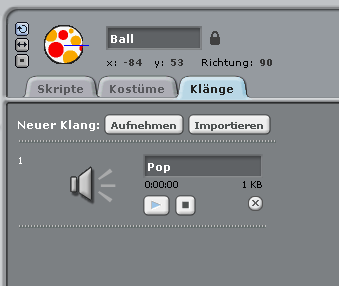
\includegraphics[width=0.6\textwidth]{images/aufgabe3_ton3.png}
\begin{itemize}
\item[13.] Klick auf den Klang-Panel, wähle die \textit{spiele Klang}-Kachel und ziehe sie unter die \textit{verstecke dich}-Kachel in dem Ball Sprite Skript-Editor.
\end{itemize}
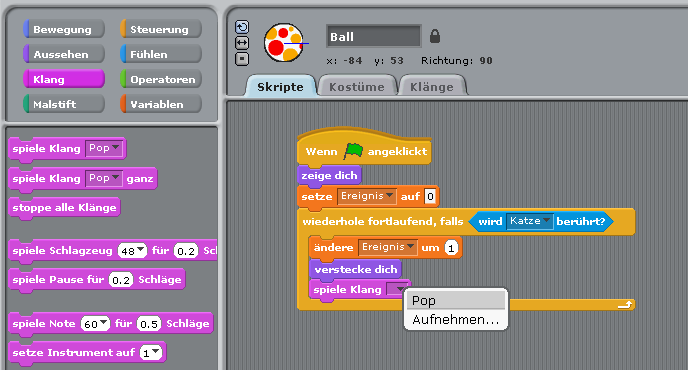
\includegraphics[width=0.6\textwidth]{images/aufgabe3_ball3.png}
\begin{itemize}
\item[14.] Klicke auf den grünen Pfeil und teste ob du etwas hörst, sobald deine Figur den Ball berührt.
\end{itemize}


\subsection{Kopiere Objekte}
\begin{itemize}
\item[15.] Sobald du zufrieden bist mit deinen Ball-Sprites und den dazugehörigen Skripten, klicke auf das Stempel-Tool, um das gewünschte Sprite zu kopieren. So kannst du die Bälle vermehren und das dazugehörige Verhalten gleich mit.
\item[16.] Kopiere die Bälle und ordne Sie innerhalb des Labyrinths an.
\end{itemize}
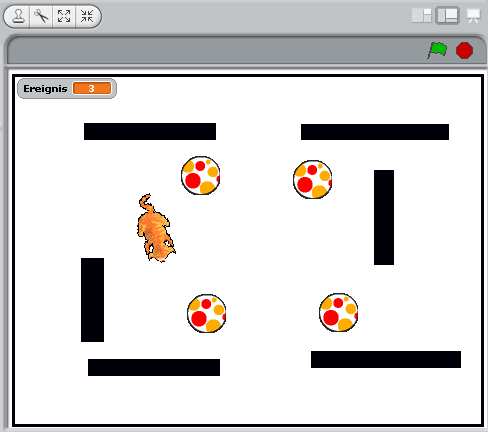
\includegraphics[width=0.6\textwidth]{images/aufgabe3_vier_baelle.png}

\subsection{Füge Hintergrundmusik hinzu}
\begin{itemize}
\item[17.] Du kannst Musik in dein Spiel einfügen. Scratch spielt alle Lieder mit der Dateiendung .mp3 und .wav ab.
\item[18.] Klicke auf das Bühnen Icon.
\item[19.] Klicke auf das Klang-Panel und befolge Anweisungen aus Schritt 3.
\item[20.] Ziehe die \textit{Wenn grüne Flagge geklickt}-Kachel in das Skript-Panel.
\item[21.] Hänge daran, die \textit{wiederhole fortlaufend}-Kachel.
\item[22.] Füge in diese den Klang ein.
\item[23.] Drücke die grüne Flagge und teste dein Spiel.
\end{itemize}